\chapter{Data and Methods} \label{chap:data}

\begin{figure}

\centering
\includegraphics[width=.5\textwidth]{reach}
\caption{Size of targetable population (reach estimate) with the targeting options selected in Figure \ref{fig:ad_interface} i.e. women living in the United States, between the ages of 13 and 35, who are interesting in engineering.}
\label{fig:reach}

\end{figure}

\begin{figure}
\centering
\includegraphics[width=.8\textwidth]{ad_interface}
\caption{Screenshot of Facebook's Ads Manager interface showing some of the major functionalities available. Geographical location, age and gender have been specified. An elaborate list of targeting options are available through the cascading drop-down menus under ``Detailed Targeting". Here, the category ``Engineering" has been selected.}
\label{fig:ad_interface}

\end{figure}

In our work, we draw from Facebook advertising data to produce estimates of the number of users with particular demographics and interests. In this document, we broadly explain the structure of Facebook's advertisement ecosystem, the data we gather from the system, and the techniques we use to analyze it.

% In this section, we broadly explain the structure of Facebook's advertisement ecosystem, the data we gather from the system, and the techniques we use to analyze it.

\section{Mechanism of Data Collection} \label{sec:fb_ad_eco}

% LATER: for thesis draft, explain the scale of how many people are affected by these ads and how important all of it is to Facebook.
As the world's largest social network\footnote{\url{https://www.weforum.org/agenda/2017/03/most-popular-social-networks-mapped/}}, Facebook's targeted advertising system allows marketers and businesses to target ads to its users by their demographic attributes, location, as well as interests and internet behaviors that it has inferred about them (Figure~\ref{fig:ad_interface}). The system reports how many people would fit the specified criteria -- which it refers to as the \textit{reach estimate} (Figure~\ref{fig:reach}).

The ability of the platform to a) simultaneously target users by both their demographic and behavioral attributes; and b) to provide reach estimates prior to actually launching the ads, makes it a useful tool for understanding the characteristics of a population -- or at least what Facebook \textit{thinks} they are.

Using the social network's ad system, we can issue very specific queries such as ``the number of women between the ages of 25 and 29 interested in online shopping" or ``the number of African-American men managing small business pages on Facebook", and then compare the given reach estimates across demographic groups -- all without ever launching an ad.

Facebook provides multiple tools to target advertisements on the social network: uploading a list of emails or phone numbers for users to target, matching people who are similar to people who clicked on a previous advertisement, and finding people with a given set of features ranging from demographic variables such as gender and relationship status to interests such as anime movies and hip hop music. This third advertising method is named \textit{Core Audiences}\footnote{\url{https://www.facebook.com/business/products/ads/ad-targeting}}.

In our work we utilize the Marketing API to specify combinations of Core Audience features (e.g., demographics, interests, and geographic locations) and obtain reach estimates for these combinations. That is, we obtain estimates of how many users with a given set of demographics, in a given location, Facebook has assigned a particular interest.

\subsection{Available Variables} \label{subsec:targeting_options}

Figure \ref{fig:ad_interface} shows the structure of Facebook's \textit{Ads Manager} page, where marketers can construct core audiences for advertisement campaigns. We see that the interface provides the option to target by location, age, gender, language and a wide array of options under the ``Detailed Targeting" section.

\textbf{Location.} For location based targeting, Facebook provides the option to target countries, regions comprising multiple countries (e.g. Asia or the European Economic Area), regions within countries such as provinces or states, cities, ZIP codes, as well as congressional districts in the United States. It also allows radius targeting by dropping a pin at a particular address and specifying a target radius as small as 1 kilometer around it. For all geographic options, advertisers are able to target people who either live in the area, have recently traveled there, are currently traveling to the area, or all of the above.

\textbf{Demographics.} You can choose to advertise to people aged 13 - 100 years and to people who are Male, Female, or Other (the advertising interface groups non-binary genders into a single category). Age and gender are both directly self-reported variables. 

Under detailed targeting, you can also select a number of other demographics including education level, employment, ethnic affinity, and expat status. Education is self reported, but all other demographic variables are inferred. Note that income data is no longer available, as this data was provided by third parties and Facebook has discontinued use of that data.

\textbf{Interests} Under detailed targeting you can also specify various different types of interests\footnote{Note that while Facebook has groupings under detailed targeting called "Behaviors" and "Interests" these categories may at time contain demographics (e.g., ethnic affinity, expat status), or interests (e.g., in education) may be placed in the ``Behaviors'' category, and vise versa. Thus, we manually evaluate all of the features, and examine advertisements that have been targeted using them, to better understand the true representation of a particular feature.}, which are grouped by themes such as ``Fitness and wellness", ``Hobbies and activities", ``Business and Industry'' and etc. The ``Business and Industry'' category includes, for example, ``Higher Education'' which we find appears to proxy for an interest in education.

\textbf{Behaviors} Finally, under detailed targeting you can also specify behaviors. For example, the type of device or operating system a person users or their purchasing behaviors.

\textbf{Open Text} In addition to the features characterized under these three categories, Facebook also automatically indexes other interests across the platform which advertisers can search by inputting free text. Many of these features have been observed to be directly related to pages on the social network and are explained in the Ads Manager as targeting ``people who have expressed an interest in" or ``like pages related to" the particular feature.

It is also important to note that the list of these targetable features is not static. It is subject to moderation if the users report a feature in the list as inappropriate. As an example, this public moderation practice has previously led to Facebook renaming the ethnic affinity feature \cite{propublica_fb_ethnic_affinity_again}, and removing problematic anti-semitic ad categories that were automatically indexed by the ad system \cite{propublica_jew_hater_study}. These regular changes to the features warrant caution while collecting data from the platform.

\section{Dataset} \label{subsec:data_collected}
We create a dataset of reach estimates corresponding to the number of people with a particular set of demographics who Facebook reports are interested in a particular thing or behave in a particular way. We focus exclusively on the United States as it has high Facebook penetration and is the only region where Facebook infers user ethnicity.

%Demographically, we choose to focus on age, gender, ethnicity and education; we discontinue using education for our later analyses because of poor quality estimates from the ad platform (more detail in Section \ref{sec:fb_quality}).

%For the advertisement estimates, we query the API for the interest each demographic group shows in the ad-targeting features. We limit our estimates to the United States as it is a high internet penetration country, and also the only region where Facebook infers user ethnicity -- or ``Multicultural Affinity" as the Ads Manager calls it.

\textbf{Demographics:} We collect data split by age, gender, ethnicity, and education. Since Facebook doesn't have an explicit White ethnicity attribute, we obtain this estimate by excluding all other ethnic groups recorded by the platform. We query for age by breaking down the ages into five year bins starting from 15 until ``60+", which is the maximum targetable age on the platform.

\textbf{Behaviors and Interests:} We collect the full list of 323 interests and 264 behaviors specified in the advertising interface. For each interest and behavior we collect a) the total number of people interested in the attribute; and b) the number of people from each demographic group interested in the attribute.

%later you'll end up talking about custom sets?% 

\subsection{Quality of Data} \label{sec:fb_quality}
Since our study focuses on Facebook's ad-targeting features and their associations along different demographic dimensions, it is imperative that Facebook's estimates for these demographic variables are reliable. Gender, age and education are self-reported on the social network, while ethnicity (available only in the United States) is an inferred feature. Errors might arise either due to faulty self-reporting or due to problems in Facebook's inference mechanism.

As of the time of this writing, the Ads Manager reports that 240 million people who live in the United States are targetable with Facebook ads. To understand the scale of this penetration, we stratify this estimate by the ACS population estimate for each state and observe what fraction of the population in each state is targetable. Figure \ref{fig:rep_map} shows the fraction of the population in each state that is targetable with Facebook's targeted ads. We find that the lowest penetration is in New Jersey with 58.13\% of the population being targetable. The average penetration over all states is 69.45\%. This helps illustrate the scale of the platform in a country like the U.S. where a large fraction of the population is reachable and can be studied with advertisement data.

% ==== map figure ====
\begin{figure}
\centering
\includegraphics[width=\textwidth]{representation}
\caption{State level penetration of Facebook advertisements in the United States. In every state, at least half of the population is reachable with targeted advertising.}
\label{fig:rep_map}
\end{figure}
% ====

\if(
% === correlation figures ===
% === for smaller figure widths, this would put images side by side ===
\begin{figure}
    \centering
    \subfloat[Men. $\rho=0.996 \;(p < 10^{-20})$; $R^2=0.992$.]{{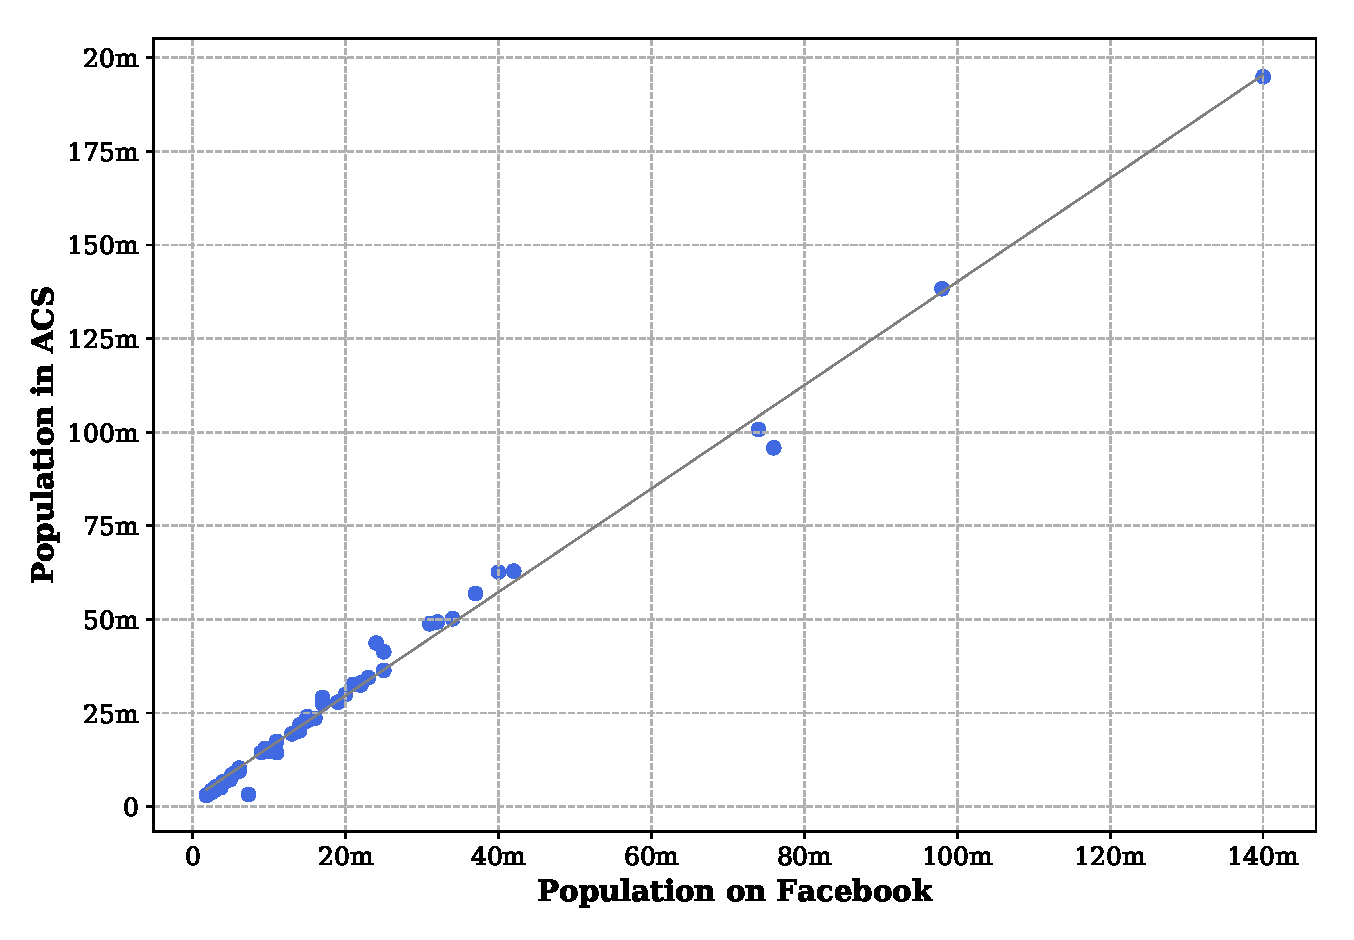
\includegraphics[width=.75\textwidth]{men_corr} }}
    \qquad
    \subfloat[African Americans. $\rho=0.983 \;(p < 10^{-20})$; $R^2=0.966$.]{{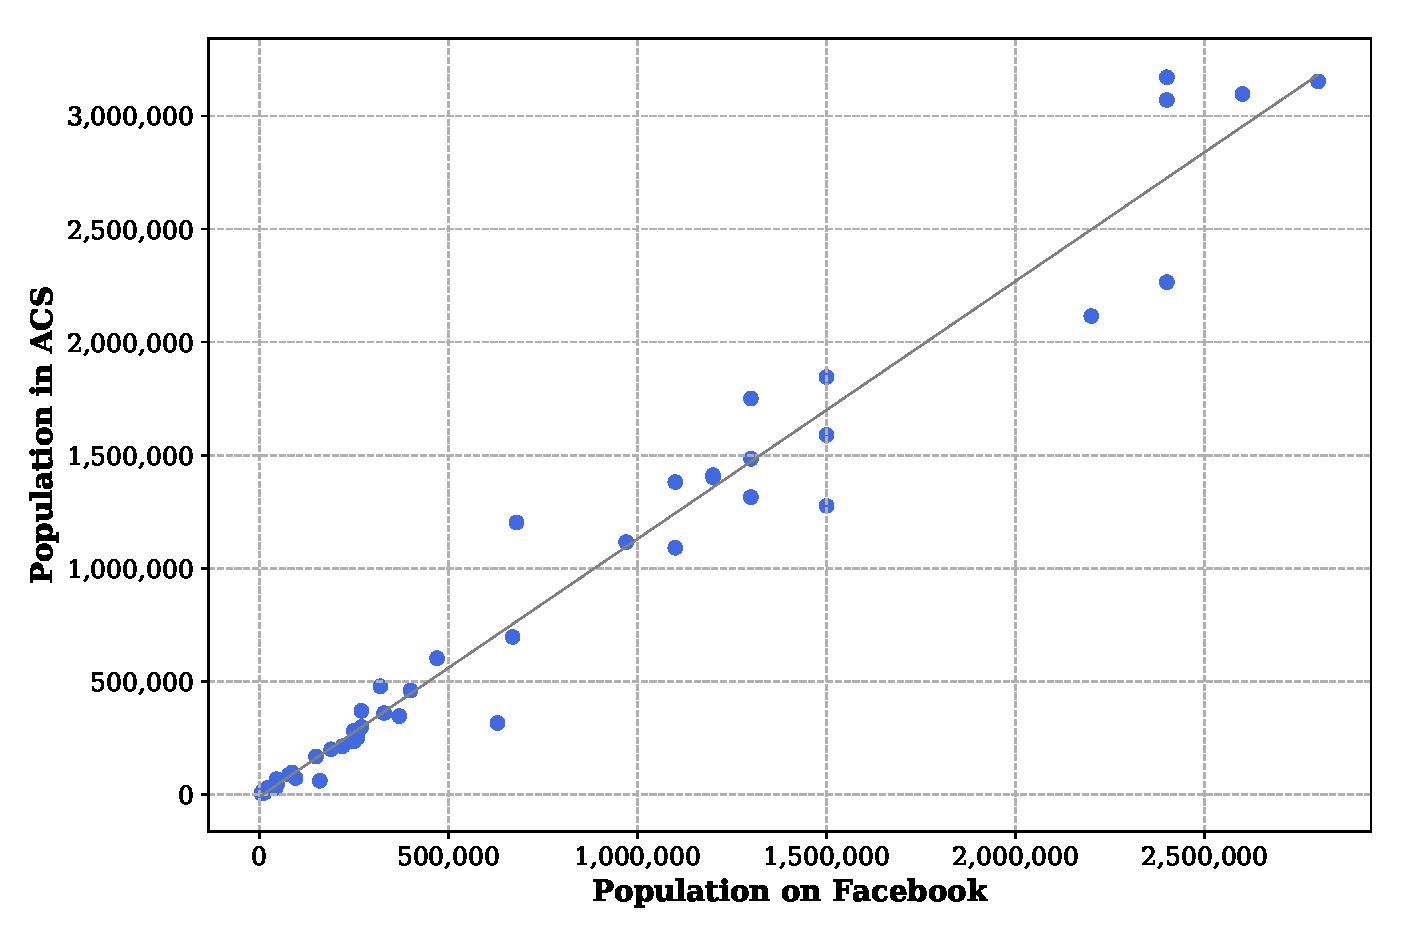
\includegraphics[width=.75\textwidth]{black_corr} }}

    \caption{Gender and ethnicity estimate comparisons from Facebook with ground truth data from the American Community Survey (ACS). Above: Comparison for gender estimates; the number of men in each state is shown. Below: Comparison for ethnicity estimates; the number of African Americans in each state is shown. The grey lines show a linear regression model fit to the estimates from Facebook. The correlation coefficient $\rho$, and the coefficient of determination $R^2$ for the linear model have been reported.}
    \label{fig:corrs}
\end{figure}
% ====
)\fi

% To evaluate the quality of demographic estimates, we compare Facebook's estimates against ground truth data obtained from the developer API provided by ACS\footnote{\url{https://www.census.gov/data/developers/data-sets.html}}.

To investigate the quality of demographic estimates in our data, we compare the Facebook demographic estimates to ground truth data from the American Community Survey's 2016 5-year estimates. Table \ref{tab:comparison} shows the comparison of gender, ethnicity, education and age estimates in the Facebook dataset to the ACS figures. While $\chi^2$ proportion tests show significant differences in the estimates for all variables, when observing the effect size of these differences we find that meaningful differences (Cohen's $h$>0.2 (small)) are observed for only one age group and for educational attainment. Given the size of the educational attainment differences (medium) we exclude educational attainment from our analysis. 

% ====== representation table =======
\begin{table}
\centering
\begin{tabular}{c | c | c | c | c} 
\toprule
\textbf{Variable} & \textbf{Value} & \multicolumn{3}{c}{\textbf{\%}}\\
& & \textbf{Facebook} & \textbf{ACS} & \textbf{$\Delta$}\\
 \hline
\textbf{Gender} & Male & 45.83 & 49.21 & -3.38\\
& Female & 54.16 & 50.78 & +3.38\\
 \midrule
 \textbf{Ethnicity} & White & 64.58 & 61.95 & +2.63\\
 & Black & 14.16 & 12.63 & +1.53\\
 & Asian & 3.08 & 5.21 & -2.13\\
 & Hispanic & 13.75 & 17.32 & -3.57\\
 \midrule
 \textbf{Completed education} & Less than high school & 3.16 & 10.09 & -6.93*\\
 & High school & 17.08 & 21.41 & -4.33\\
 & College & 31.25 & 13.61 & +17.64**\\
 & Graduate school & 4.11 & 7.71 & -3.6\\
 \midrule
 \textbf{Age} & 15-19 & 5.83 & 6.69 & -0.86\\
 & 20-24 & 12.91 & 7.09 & +5.81\\
 & 25-29 & 13.75 & 6.89 & +6.85*\\
 & 30-34 & 10.83 & 6.69 & +4.13\\
 & 35-39 & 10.41 & 6.29 & +4.11\\
 & 40-44 & 8.33 & 6.39 & +1.93\\
 & 45-49 & 8.33 & 6.59 & +1.73\\
 & 50-54 & 7.08 & 6.99 & +0.08\\
 & 55-59 & 6.25 & 6.69 & -0.44\\
 & 60+ & 14.16 & 20.39 & -6.23\\ 
 \bottomrule
\end{tabular}
\caption{Percentage demographic makeup of Facebook's population in the United States, compared with ground truth data from the American Community Survey (ACS). The difference in Facebook is shown as $\Delta$. $\chi^2$ test of proportions yields $p < 0.001$ for all measurements, with small effect size (Cohen's $h < 0.2$) for unmarked differences. *$h = 0.2$; **$h = 0.4$.}
\label{tab:comparison}
\end{table}
% =============

\section{Methods for Analysis} \label{sec:methods}
We use three different metrics to compute answers to the following three types of questions that we can ask about our data:

\begin{enumerate}
\item What proportion of people in a given demographic group have a particular interest or behavior?
\item Are members of a particular demographic group more likely to be inferred as having this interest or behavior than the general population?
\item Are members of a particular demographic group more likely to be inferred than those in another demographic group?
\end{enumerate}

To answer the first question, we look at what fraction of a group's population is interested in an attribute according to Facebook. We refer to this ratio as the \textit{penetration} of the attribute in the group. For a demographic $d$ and feature $f$ on the platform, we define penetration as

\begin{equation}
\text{penetration}_g(d, f) = \frac{n_g(d, f)}{n_g(d)},
\label{eq:pen}
\end{equation}

where $n_g(d)$ is the reach estimate (i.e. number of people targetable) by specifying demographic $d$ alone on the platform. $n_g(d, f)$ refers to the intersection of populations targetable with demographic $d$ and feature $f$. Because of the nature of the ad ecosystem, a geographical location of the audience must always be specified, which is shown here as $g$.

Equation \ref{eq:pen} gives us a simple statistic for the association of each demographic in our dataset to the attributes on the platform. To answer the second question of whether a group is more or less likely to be inferred than the general population, we build on top of penetration and define the notion of \textit{affinity}. We define the affinity for a demographic group $d$ towards a targetable feature $f$ as

\begin{equation}
\text{affinity}_g(d, f) = \frac{n_g(d, f)}{n_g(d)} - \frac{n_g(f)}{N_g}.
\label{eq:aff}
\end{equation}

Following similar notation, here $n_g(f)$ refers to the reach estimate for feature $f$ without specifying any demographic; $N_g$ denotes total population in region $g$ according to Facebook. All estimates involved in these computations are obtained with the data collection process described in Section \ref{subsec:data_collected}.

A large positive affinity would indicate that members of demographic $d$ are considered much more likely by the ad platform to be interested in feature $f$, as compared to the general population in region $g$. Analogously, a large negative value would mean Facebook does not associate group $d$ with the feature $f$ and some other subgroup of the population in $g$ is more highly interested.

\if(
where $n_g(d)$ and $n_g(f)$ are the reach estimates (i.e. number of people targetable) by specifying demographic $d$ and feature $f$ alone. $n_g(d, f)$ refers to the intersection of populations targetable with $d$ and $f$. Because of the nature of the ad ecosystem, a geographical location of the audience must always be specified, which is what the $g$ in the subscript refers to. Consequently, $N_g$ is the total population in region $g$ according to Facebook. All these estimates are obtained with the data collection process described in Section \ref{subsec:data_collected}.
)\fi

For answering the third question of whether one demographic is more likely than another to be inferred for an attribute, we compare the affinity of the attribute for both groups. We refer to the difference in affinity (or alternatively, penetration) for two groups $d_1$ and $d_2$ as their \textit{disparity} on targeting feature $f$,

\begin{align*}
\text{disparity}_g(d_1, d_2, f) &= \text{penetration}_g(d_1, f) - \text{penetration}_g(d_2, f)\\
&= \frac{n_g(d_1, f)}{n_g(d_1)} - \frac{n_g(d_2, f)}{n_g(d_2)}. \addtocounter{equation}{1}\tag{\theequation}
\label{eq:disparity}
\end{align*}

Naturally, for two groups $d_1$ and $d_2$ that have large disparity for a feature $f$, Facebook has a very different understanding of their interest in $f$. As a result, a higher fraction of the group with the larger affinity would end up seeing content related to $f$. Moreover, targeted ads also present the opportunity to expand these differences. By disproportionately showing ads for attributes that might be relevant for both demographics, disparities might reinforce themselves over time. Therefore, having a notion of disparity between two demographics allows us to observe the differences Facebook believes these groups have.

It also allows us to be more rigorous by performing statistical testing on the disparity and see whether the differences are statistically significant. For a set of targeting features $F$ and a feature $f^* \in F$ with positive value of the disparity statistic $T = \text{disparity}_g(d_1, d_2, f^*)$, we are able to compute the p-value with a maximum likelihood estimate as

\begin{align*}
p &= \Pr[\; \text{disparity}_g(d_1, d_2, f) \geq T \;]\\[.3em]
&= \frac{\big|\{f \in F \; | \; \text{disparity}_g(d_1, d_2, f) \geq T\}\big|}{|F|} \addtocounter{equation}{1}\tag{\theequation}
\label{eq:p_val_positive}
\end{align*}

In our situation, $F$ is the set of all features that we have gathered from Facebook's APIs. Similarly, for negative values of the disparity statistic, we look towards more extreme negative values to compute the p-value,

\begin{align*}
p &= \Pr[\; \text{disparity}_g(d_1, d_2, f) \leq T \;]\\[.3em]
&= \frac{\big|\{f \in F \; | \; \text{disparity}_g(d_1, d_2, f) \leq T\}\big|}{|F|} \addtocounter{equation}{1}\tag{\theequation}
\label{eq:p_val_negative}
\end{align*}

This simple but useful way of significance testing gives us a clear idea of the strength of any difference in feature disparities. Using this framework, we are able to answer questions like whether there are significant differences between men and women in Facebook's inference of professional features such as engineering; or what kind of industries the ad platform associates most with African Americans. Moreover, we are able to do this without launching any malicious or harmful ads and only through the reach estimates provided in the Ads Manager.